\documentclass[11pt,preprint, authoryear]{article}

\pagestyle{plain}

\usepackage{lmodern}

% spacing passed through from .Rmd doc
\usepackage{setspace}
\setstretch{1.5}

% Wrap around which gives all figures included the [H] command, or places it "here". This can be tedious to code in Rmarkdown.
\usepackage{float}
\let\origfigure\figure
\let\endorigfigure\endfigure
\renewenvironment{figure}[1][2] {
    \expandafter\origfigure\expandafter[H]
} {
    \endorigfigure
}

\let\origtable\table
\let\endorigtable\endtable
\renewenvironment{table}[1][2] {
    \expandafter\origtable\expandafter[H]
} {
    \endorigtable
}

\usepackage{ifxetex,ifluatex}
\usepackage{fixltx2e} % provides \textsubscript
\ifnum 0\ifxetex 1\fi\ifluatex 1\fi=0 % if pdftex
  \usepackage[T1]{fontenc}
  \usepackage[utf8]{inputenc}
\else % if luatex or xelatex
  \ifxetex
    \usepackage{mathspec}
    \usepackage{xltxtra,xunicode}
  \else
    \usepackage{fontspec}
  \fi
  \defaultfontfeatures{Mapping=tex-text,Scale=MatchLowercase}
  \newcommand{\euro}{€}
\fi

\usepackage{amssymb, amsmath, amsthm, amsfonts}

\DeclareMathSizes{24}{26}{22}{22}

\usepackage[round]{natbib}
\bibliographystyle{natbib}
\def\bibsection{\section*{References}} %%% Make "References" appear before bibliography

% package for nice tables
\usepackage{longtable}

% package for ruling lines in tables
\usepackage{booktabs}

% set margins
\usepackage[left=3.5cm, right=2cm, top=30mm ,bottom=2cm, includefoot]{geometry}
\usepackage{fancyhdr}
\usepackage[bottom, hang, flushmargin]{footmisc}
\usepackage{graphicx}
\numberwithin{equation}{section}
%\numberwithin{figure}{section} % commented out because it messes up figure numbering
%\numberwithin{table}{section} % commented out because it messes up table numbering
\setlength{\parindent}{0cm}
\setlength{\parskip}{1.3ex plus 0.5ex minus 0.3ex}
\usepackage{textcomp}
\renewcommand{\headrulewidth}{0pt}

\usepackage{array}
\newcolumntype{x}[1]{>{\centering\arraybackslash\hspace{0pt}}p{#1}}

\usepackage{hyperref}
\hypersetup{breaklinks=true,
            bookmarks=true,
            colorlinks=true,
            citecolor=blue,
            urlcolor=blue,
            linkcolor=blue,
            pdfborder={0 0 0}}
						
\urlstyle{same}  % don't use monospace font for urls
\setlength{\parindent}{0pt}
\setlength{\parskip}{6pt plus 2pt minus 1pt}
\setlength{\emergencystretch}{3em}  % prevent overfull lines
\setcounter{secnumdepth}{5}

% Use protect on footnotes to avoid problems with footnotes in titles
\let\rmarkdownfootnote\footnote%
\def\footnote{\protect\rmarkdownfootnote}
\IfFileExists{upquote.sty}{\usepackage{upquote}}{}

% pass through extra packages specified by user
\usepackage{bm}

%%%%%%%%%%%%%%%%%%%%%%%%%%%%%%%%%%%%%%%%%%%
%%%%%%%%%%%%%%%%%% EDIT TITLE %%%%%%%%%%%%%%%%%%
%%%%%%%%%%%%%%%%%%%%%%%%%%%%%%%%%%%%%%%%%%%

% change title format to be more compact
\usepackage{titling}

% create subtitle command for use in maketitle
\newcommand{\subtitle}[1]{
  \postauthor{
    \begin{center}\large#1\end{center}
    }
}

\setlength{\droptitle}{-1em}
\pretitle{\vspace{\droptitle}\centering\Huge}
\posttitle{\par\vskip 5.5em}

\title{
{\scshape\Large Department of Statistics 2019}\\
{\vskip 2.5em \scshape Predicting Community Engagement with Questions for Chronological
StackOverflow Datasets}\\
%{\includegraphics{lse.png}} % if you want to include LSE logo
}

\preauthor{\centering\LARGE}
\postauthor{\par\vskip 4em}

\author{Candidate Number: 10140}
\subtitle{\vspace{4em} Submitted for the Master of Science, London School of Economics,
University of London} % comment this out and you get *Missing \begin{document}*

\predate{\centering\Large}
\postdate{\par}

\date{\scshape August 2019}

\usepackage{color}
\usepackage[usenames,dvipsnames,svgnames,table]{xcolor}
\usepackage{hyperref}
\hypersetup{
     colorlinks = true,
     citecolor = gray
}

\usepackage{tocloft}

\renewcommand{\cftsubsecfont}{\normalfont\hypersetup{linkcolor=black}}
\renewcommand{\cftsubsecafterpnum}{\hypersetup{linkcolor=black}}

%%%%%%%%%%%%%%%%%%%%%%%%%%%%%%%%%%%%%%%%%%%
%%%%%%%%%%%%%%%% BEGIN DOCUMENT %%%%%%%%%%%%%%%%
%%%%%%%%%%%%%%%%%%%%%%%%%%%%%%%%%%%%%%%%%%%

\begin{document}

% Header and Footers
\pagestyle{fancy}
\chead{}
\rhead{}
\lfoot{}
\rfoot{} 
\lhead{}
%\rfoot{\footnotesize Page \thepage\ } % "e.g. Page 2"
\cfoot{\footnotesize \thepage\\}

% i, ii, iii etc. page numbering
\pagenumbering{roman}

\maketitle

\thispagestyle{empty}

\clearpage

\setcounter{page}{1}

% table of contents, list of figures and tables
\renewcommand{\contentsname}{Table of Contents}
\hypersetup{linkcolor=black}
\tableofcontents
\newpage
\hypersetup{linkcolor=black}
\listoffigures
\newpage
\hypersetup{linkcolor=black}
\listoftables
\hypersetup{linkcolor=black}
\newpage

\section*{Summary}

Formulating constructive questions and receiving answers to these
questions is crucial to how we examine, learn from and critically
analyse the world around us. The evolution of the world wide web and the
technologies that have emerged with it have given us an unprecendented
ability to engage with and learn from individuals around the world, and
while substantial attention has been dedicated to finding the right
answers (just ask Google), comparitively less has been devoted to how we
can improve the constructiveness of our questions. The domain of online
question-answer (Q\&A) communities is one setting where relevant and
well-researched questions are of particular importance, not least
because domain expert resources are often scarce compared to unrelenting
cascades of new questions (a problem known as information overload).
This research builds on the small collection of work aimed at questions
in online Q\&A communities, and analyses chronological datasets from
\href{https://stackoverflow.com/}{StackOverflow.com}, not only one of
the largest Q\&A communities on the internet, but the 41st most popular
website according the \href{https://www.alexa.com/topsites}{Alexa rank}
at the time of writing. Using only textual question content available at
the time questions are initially submitted, I construct models to
predict the community-granted score for each question which I consider a
comprehensive measurement of community engagement. Contrary to similar
prior work, I find that topic models lead to \textbf{almost no
improvement in prediction metrics across datasets}. My research shows
that there is still much work to be done to accurately predict community
engagement in online Q\&A fora, let alone \emph{future} community
engagement. Nevertheless, this research serves as a stepping stone in
addressing information overload in online Q\&A communities by informing
questioners of how their questions will be acknowledged, potentially
nudging them to enhance their questions before adding demand to these
communities and improving the functioning of these platforms
substantially. (307)

\clearpage

% 1, 2, 3 etc. page numbering
\pagenumbering{arabic}

\newpage

\section{\texorpdfstring{Introduction
\label{Intro}}{Introduction }}\label{introduction}

Modern interpersonal communication technologies made possible by the
internet have afforded us an exceptional level of connection and
engagement with the world. Billions of individuals now interact online
instantly, not only with people that they know, but with strangers
millions of miles away. One avenue of online interaction that has become
an extremely popular way in which users share knowledge about diverse
and nuanced subject matter is question-and-answer (Q\&A) websites such
as Yahoo! Answers, Quora, the StackExchange family and forums of Massive
Online Open Courses (MOOCs). These websites serve as dynamic, engaging
platforms where users seek answers to and discussions on complex and
technical questions that modern search engines are evidently yet unable
to fully address.

Producing relevant, well-researched and high-quality questions in these
online Q\&A fora is especially valuable, not least since these platforms
suffer in particular from a low ratio of expert resources to volume of
new questions - an example of the problem known as \emph{information
overload} (Eppler and Mengis, 2004). The overarching hypothesis of this
research is that if questioners in online Q\&A fora were provided with
information specifically related to how well their questions would be
received by communities, they could then iterate to ``increase the
signal'' of their questions before exerting demand on community
resources, mitigating the problem of information overload. If this were
possible, it would no doubt benefit questioners in that they would
effectively garner expert answers to their improved questions, but also
entire communities as overall functioning and efficiency would be
enhanced community-wide.

Predicting how positively or negatively online communities would react
to user questions in real time is a non-trivial problem however, since
these predictions would have to be made using only the information
available when new questions are formulated. This implies that
predictive models would only be able to learn from features derived from
question content, as opposed to features such user characteristics,
final webpage viewing statistics etc.

Ideally, final predictions given to questioners would also ideally be
highly granular and direct questioners towards how best to improve their
questions in the form of a recommendation system, however the aim of
this research is to progress one step from previous work on questions in
online Q\&A communities and ascertain if community engagement in online
Q\&A fora can actually be predicted with some measure of accuracy.

The broad research question for this paper can therefore be summarised
as the following:

\begin{center}
\emph{To what extent can community engagement with questions in online Q\&A communities be accurately predicted using only question content?}
\end{center}

While there is a substantial amount of literature that has addressed
online Q\&A communities, interestingly the focus has been on identifying
expert users and high quality answers rather than on questions, despite
questions being the entry point for every interaction in communities. In
an attempt to answer the research question above, I build on the small
collection of research on \emph{question quality} in online Q\&A fora
and draw heavily on work done by Ravi \emph{et al.} (2014) on the
popular computer programming community
\href{https://StackOverflow.com}{StackOverflow}. I critique and expand
the analysis of Ravi \emph{et al.} (2014) by considering a continuous
response variable measuring community engagement as opposed to binary
and analyse multiple, chronological \textbf{monthly} StackOverflow
datasets.

Since the StackOverflow online Q\&A community records an aggregation of
all community \emph{up-votes} and \emph{down-votes} for questions in a
\texttt{Score} variable, I argue that this comprehensively captures
community engagement and predict this variable using only the textual
content of questions. In line with the analysis of Ravi \emph{et al.}
(2014), I employ latent Dirichlet allocation (Blei, Ng and Jordan, 2003)
(LDA) to engineer latent topic features from question content for
predictions. I use \textbf{elastic-net} regularised regression for the
learning task and evaluate models using root-mean-square error (RMSE).

It should be highlighted that the goal of this research is quantitative
prediction rather than qualitative, causal or inferential analysis. I
leave it to further research to address more precisely the \emph{how}
and \emph{why} of community engagement in online Q\&A communities,
rather than just the \emph{if} that is explored here. To my knowledge
this research is the first of its kind to test latent topic models on a
continuous and objective measurement of online community engagement over
chronological time periods as well as have a real-life use-case,
resulting in a practical and unique contribution.

\newpage

\textbf{My findings} show that there is still much work to be done to
accurately predict community engagement in online Q\&A fora. I find that
models that include features derived from the lengths and topics of
questions do \textbf{NOT} perform better than a baseline of just average
\texttt{Score} prediction from the training question set.
\textbf{leading me to believe that in order to accurately predict future
community engagement, models need to incorporate temporal and
time-series elements.}

In the following section I discuss relevant literature in more detail.
This is followed by section \ref{Method} which discusses the data,
explores and validates my choice of the \texttt{Score} variable as an
objective measurement of community engagement and describes the
predictive model used. Section \ref{Results} presents and discusses the
results, section \ref{Recom} explores some recommendations for areas of
further research and finally section \ref{Concl} makes some concluding
remarks.

\newpage

\section{\texorpdfstring{Literature Review
\label{Lit}}{Literature Review }}\label{literature-review}

\subsection{Question-Answer
Communities}\label{question-answer-communities}

There is a substantial collection of research that has investigated
online Q\&A communities. Prior work has addressed answer quality (Jeon
\emph{et al.}, 2006; Shah and Pomerantz, 2010; Tian, Zhang and Li,
2013), satisfaction of questioners (Liu, Bian and Agichtein, 2008) and
the behaviour of highly productive, expert community members (Riahi
\emph{et al.}, 2012; Sung, Lee and Lee, 2013). Two common frameworks for
prior work has been the optimisation of routing questions to experts (Li
and King, 2010; Li, King and Lyu, 2011; Zhou, Lyu and King, 2012; Shah
\emph{et al.}, 2018), and matching questions in accordance with answerer
interest in the form of a recommendation system (Wu, Wang and Cheng,
2008; Qu \emph{et al.}, 2009; Szpektor, Maarek and Pelleg, 2013).

My research differs from this previous work on Q\&A fora in two
respects. Firstly, I focus on questions rather than user or answer
characteristics, not only because they have received substantially less
attention in the literature, but because it has been shown that question
quality can substantially impact the quality of answers (Agichtein
\emph{et al.}, 2008). Questions in online Q\&A fora are also the initial
event that all community engagement follows from and thus maximising
positive community engagement with questions will almost certainly
improve the evolution and functioning of communities.

The second divergence from prior research is the framework in which this
research is placed. I choose a framework of community engagement and
interaction with user actions rather than the systems-based optimisation
of question-answer routing and matching and instead concentrate on how
questioners can be nudged to improve the content of their questions
before encumbering community resources.

\textbf{Community engagement is a rather broad term in literature
ranging across fields and disciplines, but I have not found any
literature relating to community engagement in the context of online
Q\&A fora.}

With the promise of this real-life application which significantly
benefit both questioners and communtities, it remains to be seen if
community engagement in online Q\&A fora can be successfully predicted.
Owing to a large overlap between this goal and the literature on
predicting question quality in online Q\&A communities, I discuss this
literature next.

\subsection{Question Quality}\label{question-quality}

Naturally, community engagement and question quality go hand in hand:
high quality questions will no doubt lead to positive community feedback
in the form of many up-votes, answers and discussion promoting comments.
I argue later point that \emph{community engagement} is a more accurate
and thorough definition of what the following literature claims to
measure, however for the sake of discussion I will refer to
\emph{question quality} here as well.

A recent line of work has looked at predicting question quality in the
large Q\&A community \href{http://answers.yahoo.com}{Yahoo! Answers}
(Agichtein \emph{et al.}, 2008; Bian \emph{et al.}, 2009; Li \emph{et
al.}, 2012) - a dataset which has metrics for assessing answer quality
in the form of answer up-votes, however regrettably lacks a similarly
community-attributed and objective metric for question quality. This has
resulted in subjective attempts to define question quality: Agichtein
\emph{et al.} (2008) define question quality using questions' semantic
features (lexical complexity, punctuation, typos etc.), Bian \emph{et
al.} (2009) use manual labels for 250 questions and a semi-supervised
coupled mutual reinforcement framework to label a larger number of
questions, and Li \emph{et al.} (2012) combine the number of answers,
number of tags, time until first answer, author judgement and domain
expertise to construct their ground truth.

Fortunately, the StackOverflow datasets that I analyse are rich in
objective community-attributed metrics such as question up- and
down-votes, comments, and views, all over and above community answers
themselves. These metrics are objective in the sense that they do not
require construction or labeling form the researchers' side, and
subsequently allow for a large collection of questions to be analysed
automatically.

Another aspect of the literature that has evolved substantially over
time are the predictive models employed to predict question quality.
Previous work has modelled question quality based on the reputation of
the questioner, question categories and lexical characteristics of
questions (length, misspelling, words per sentence etc.) (Agichtein
\emph{et al.}, 2008; Bian \emph{et al.}, 2009; Anderson \emph{et al.},
2012; Li \emph{et al.}, 2012). By ignoring the actual textual and
topical content of questions and focusing on features of the questioner
however, these approaches would perform poorly on questions from new
users without a community history.

Owing to my research goal centering around predicting community
engagement for all community members, and in particular new and
inexperienced users who have a higher likelihood of receiving negative
community engagement due to poorly constructed questions, I use only
features available when a question is initially asked (and forego
features derived from user attributes). The methodology that I have thus
far laid out mirrors work done by Ravi \emph{et al.} (2014) to predict
question quality for the StackOverflow community, and so I discuss their
contributions next.

\subsection{\texorpdfstring{Ravi \emph{et al.}
(2014)}{Ravi et al. (2014)}}\label{ravi2014}

My research is based on and closely follows work done in Ravi \emph{et
al.} (2014). Ravi \emph{et al.} (2014) extract 410~049 questions between
2008 and 2009 from the coding community
\href{https://stackoverflow.com}{StackOverflow} to predict a binary
notion of question quality, i.e.~a prediction whether questions are
``good'' or ``bad''. Using features derived from the length, textual
content and latent topics in questions, they achieve accuracy levels of
approximately 70\%, substantially beating out a baseline ``popularity''
model using only question-webpage views by 10\%. Their conclusion is
that, through the use of latent topic models, they are able to
automatically predict a notion of question quality that extends beyond
just popularity.

While I will implement the same models on the \textbf{same dataset} as
Ravi \emph{et al.} (2014), I build on and diverge from their methodology
in a number of ways. The first and clearest distinction in my analysis
concerns the response variable to be predicted. Ravi \emph{et al.}
(2014) decide to construct a response variable by dividing the
community-attributed question \texttt{Score} (the aggregation of all
user up-votes and down-votes) by the number of views a question
receives, or a questions' \texttt{ViewCount}. They rightly state that
using the \texttt{Score} variable alone would risk conflating question
quality and popularity since questions that receive higher views are
more likely to be voted on. Since my research objective differs in that
I frame my research problem in terms of community engagement rather than
question quality, I use only the question \texttt{Score} as my response
variable. As will be expanded upon later, I believe this metric
comprehensively represents within-community engagement, of which
popularity and the ability to attract views is an integral component.

This leads me to another extension of the work in Ravi \emph{et al.}
(2014) that I make which concerns their treating the prediction problem
as binary classification, i.e.~predicting ``good'' versus ``bad''
questions. In predicting their composite response variable,
\texttt{Score}/\texttt{ViewCount}, they quite arbitrarily decide on a
threshold of 0.001 to distinguish between the good (above 0.001) and bad
questions (equal to 0), and analyse only a subset of 66~398 questions
(or only 16\% of the questions they extracted). I opt to use the
continuous \texttt{Score} variable \textbf{as it is}, mitigating any
arbitrary decisions on label boundaries for good and bad questions. In
this way, not only would questioners be provided with a more informative
prediction of how well a community will react to their questions, but it
is easily interpretated and understandable.

\textbf{Another way} in which I extend on the analysis in Ravi \emph{et
al.} (2014) is in considering a diverse range of communities/diverse
range of time periods for the StackOverflow dataset. \textbf{Temporal
stuff, different time periods.} Lastly, at the end of my analysis I will
split the train and test set temporally to take a step towards
predicting \emph{future} community engagement from \emph{past}
engagement, which I believe will complicate things, especially since I
do not employ a time-series model.

\textbf{More broadly}, I believe a framework of community engagement is
more robust and methodologically accurate than an interpretation of
``question quality''. I am of the opinion that question quality as a
definition is much more nuanced than the prior research has asserted,
not least because the definition of quality itself is highly subjective.
As an example, while most communities may universally value certain
aspects of questions such as legibility, coherence, relevance and
prior-research etc., there could be just as many or more question traits
that different communities value disproportionately - i.e.~closed-end
questions may be valued in the natural sciences to a greater extent
compared to say discussion-promoting questions in the social sciences.
Furthermore, a community's notion of ``quality'' could evolve over time.
A framework of community engagement as opposed to question quality
therefore allows for heterogeneity in how questions are valued across
communities and over time, yet still it still preserves common and
interpretable metrics for whether engagement is \emph{positive} or
\emph{negative}.

Since Ravi \emph{et al.} (2014) use the textual features and latent
topics extracted from question content and I will be emulating this part
of their research, I discuss topic modelling next.

\subsection{\texorpdfstring{Topic Models
\label{model_lit}}{Topic Models }}\label{topic-models}

Over the last decade and a half, Bayesian models have recently become
increasingly attractive in solving a range of structured Natural
Language Processing (NLP) prediction problems (Chiang \emph{et al.},
2010). Topic modelling is one such area where Bayesian inference has
become particularly prominent and which has been applied to NLP tasks
such as query-focused summarisation (Daumé and Marcu, 2006), deriving
concept-attribute attachments (Reisinger and Paşca, 2009), co-reference
resolution across documents (Haghighi and Klein, 2010), modeling
selection preferences (Ritter, Mausam and Etzioni, 2010) and name
ambiguity resolution (Kozareva and Ravi, 2011).

Topic models like LDA conceived by Blei, Ng and Jordan (2003) are
unsupervised generative probabilistic models that can be used on textual
documents to represent hidden topics as probability distributions over
words underneath the semantic structure of the text. One valuable use
for LDA and similar methods is thus to infer assortment of topics for a
collection of documents.

Allamanis and Sutton (2013) applied LDA to questions from the
StackOverflow dataset and proposed a three tiered technique: an LDA
model over the whole question body, another on code chunks in the
question body, and a last model on the question body without noun
phrases. Since Allamanis and Sutton (2013) do not attempt to predict a
measure of question quality or community engagement, Ravi \emph{et al.}
(2014) extend their analysis to demonstrate that inferred latent topics
are significant predictors of their measurement of question quality.

Indeed, with accuracy scores of up to 72\% in classifying high and low
quality questions, the analysis in Ravi \emph{et al.} (2014) hints
strongly at the capabilities of features derived from latent topics for
prediction. As in Allamanis and Sutton (2013), Ravi \emph{et al.} (2014)
build models to capture topical elements of questions at three levels,
however they choose 1) a global model to derive topics over all
questions, 2) a local topic model for sentence-level topics, and 3) a
Mallows model (Fligner and Verducci, 1986) for global topic structure
enforcing structural constraints on sentence topics in all questions.

Since Ravi \emph{et al.} (2014) see no substantial gains in predictive
accuracy when incorporating the Mallows model, I exclude this from my
methodology, \textbf{leaving me employing} the first two levels of the
methodology of Ravi \emph{et al.} (2014), engineering latent topic
features from questions on both the global level and local sentence
level. Following the methodology of Ravi \emph{et al.} (2014) and
extending it to a prediction on the continuous \texttt{Score} variable
which is assumed to be a measure of community engagement, I will be able
to ascertain if latent topic models are as effective in this new
learning task, and as effective over time with multiple StackOverflow
datasets. I begin the discussion of the data and thorough motivations
for my choice of the \texttt{Score} variable in the next section.

\newpage

\section{\texorpdfstring{Methodology
\label{Method}}{Methodology }}\label{methodology}

\subsection{\texorpdfstring{Data Selection
\label{Data}}{Data Selection }}\label{data-selection}

The \href{https://stackexchange.com/sites\#traffic}{StackExchange}
family of online Q\&A fora are a diverse range of over 170 community
websites covering topics from vegetarianism to quantum computing to
bicycles. Over and above the textual content of questions, of answers
and of comments posted since each community's conception, rich meta-data
on an array of community interactions is publicly available in XML files
compressed in 7-Zip format at
\href{http://archive.org/download/stackexchange}{archive.org}.

At over 11 years of age with 18~million questions, 11~million users and
9.3~million site visits a day,
\href{https://stackoverflow.com}{StackOverflow} is not only the oldest
and largest StackExchange Q\&A community, but is arguably the largest
dedicated computer programming community on the internet. After
launching in July 2008, StackOverflow has averaged 2~million questions
posted each year since 2012, encounters 6~200 new questions every day
({\textbf{???}}) and is ranked the 41st most popular website according
to Alexa Internet's ranking ({\textbf{???}}).

I choose to analyse \textbf{four monthly} StackOverflow question
datasets starting from \textbf{May 2009}. This choice broaches an aspect
of the research problem that has yet to be considered in the literature
- the temporality of online Q\&A data, and the potentially very
difficult challenge of predicting \emph{future} community engagement
from \emph{past} community engagement.

Predicting future community engagement is a particularly ambitious
endeavour since there is little doubt that how questioners formulate
questions and how communities value/engage with questions are subject to
change over time. The public and open nature of the StackOverflow
community, the dynamically evolving compositions of questioners and
registered-users comprising the community, and the volatile nature of
the computer programming field would all enmesh temporal trends into how
questions are formulated and received in the community.

By choosing a date range close to the start of the community and by
analysing short, uniform \textbf{monthly} snapshots of the StackOverflow
community, a number of key issues realting to temporal endogeneity are
addressed. Firstly, the choice of 2009 as the year of analysis ensures
that I don't include very recent questions that have not had enough time
to garner votes and views. The use of short timespans also minimises the
possibility of questions evolving over time, by increasingly distinct
groups of individuals (questioner- and question-specific variation).

In using short time-periods I also mitigate confounding aspects
regarding the community itself evolving and changing how it values and
engages with questions (community-specific variation), or the formal
structure of the community changing (community-structure variation).
Examples of the structure of the StackOverflow community changing would
include various nudges and guides that have been implemented for users
to ask better questions or the increasing ``gamification'' of the
reputation metric. Lastly, using \textbf{monthly} chronological datasets
results in minimal size differences between datasets (of which the
months from \textbf{May 2009 to August 2009} had the least size
differentials). Note that my final underlying assumption is thus that
there are no temporal elements or trends in the \textbf{monthly}
datasets I analyse, and so I do not employ time-series models, but treat
each isolated portion of the full data as a homogenous, unbiased
dataset.

The \textbf{four monthly} datasets have sizes ranging from 26~026 in
\textbf{May 2009}, to 32~998 in \textbf{August 2009}. Owing to the size
of these datasets (120~331 questions in total), I process and analyse
the data with PySpark, a Python API for the open-source
cluster-computing framework \href{http://spark.apache.org}{Apache
Spark}. Due to RAM and CPU capacity constraints on my local machine, I
rent powerful virtual machines on the
\href{https://cloud.google.com/}{Google Cloud Platform} for the modeling
section of the analysis. In the interests of transparency and
reproducibility, the entire PySpark codebase for the processing and
modelling of the data done can be found at
\url{https://github.com/BCallumCarr/msc-lse-thesis/}.

Since the StackOverflow dataset is also publicly and freely available
for selective querying on
\href{https://cloud.google.com/bigquery}{Google Big Query}, I use this
tool to download my variables of interest from \textbf{May to August
2009} in JSON files and convert to
\href{https://parquet.apache.org}{Parquet} format. The following
resulting variables are of interest to my analysis:

\setstretch{0.95}

\begin{itemize}
\item
  \texttt{Score}: An aggregate variable calculated from the difference
  between registered-user granted up-votes and down-votes for a question
\item
  \texttt{ViewCount}: A counter for the number of page views a question
  receives (from both registered and non-registered users)
\item
  \texttt{Title}: The text of the question title
\item
  \texttt{Body}: The text of the question body
\item
  \texttt{CreationDate}: A datetime variable indicating when the
  question was initially posted
\item
  \texttt{AnswerCount}: The number of answers a question has received
\item
  \texttt{CommentCount}: The number of comments a question has received
\item
  \texttt{FavoriteCount}: The number of times registered-users have
  favourited a question
\item
  \texttt{AcceptedAnswerId}: An indication of which answer the
  question-asker has selected as accepted
\item
  \texttt{LastEditDate}: A datetime variable indicating when the post
  was last edited
\item
  \texttt{ClosedDate}: A datetime variable indicating if a question was
  closed
\end{itemize}

\setstretch{1.25}

\textbf{In the following section I validate my choice of the
\texttt{Score} variable as a comprehensive and informative measurement
of community engagement to be used as a response to predict on.}

\subsection{Capturing Community
Engagement}\label{capturing-community-engagement}

\subsubsection{\texorpdfstring{Justification of the \texttt{Score}
Variable
\label{Vars}}{Justification of the Score Variable }}\label{justification-of-the-score-variable}

There are a number of ways that StackOverflow members engage and
interact with each other aside from the fundamental activities of
asking/answering questions and up-/down-voting questions and answers.
Questioners are able to indicate that an answer has explicitly answered
their question, users can ``favourite'' questions and there are also
further privileges for users with enough site \emph{reputation}.

Although questions on all StackExchange sites are open to the public,
posting a question in a community requires registration with an email
address and a username - once registered, users start with a
\emph{reputation} level of 1. According to the guidelines of the
StackOverflow community, reputation is a ``rough measurement of how much
the community trusts you; it is earned by convincing your peers that you
know what you're talking about'' (see
\url{https://meta.stackexchange.com/questions/7237/how-does-reputation-work}).
Key reputation levels for this analysis include:

\setstretch{0.95}

\begin{itemize}
\item
  1: Users can ask questions and contribute answers
\item
  15: Users can up-vote questions and answers
\item
  15: Users can flag posts to bring them to the attention of the
  community
\item
  50: Users can comment on questions and answers
\item
  125: Users can down-vote questions and answers
\item
  2000: Users can immediately edit any question or answer
\item
  3000: Users can vote to close questions that are off-topic, unclear,
  duplicates, too-broad or too opinion-based
\end{itemize}

\setstretch{1.25}

Despite the fact that there are many proxies for community engagement
and that they are all richly recorded in the data, there are few if any
that match the holistic, comprehensive and informative nature of the
\texttt{Score} variable.

Since the \texttt{Score} variable is the aggregation of all registered
community members' up-votes and down-votes (in accordance with their
reputation levels) it is able to register both positive (up-votes),
negative (down-votes) and neutral (abstentions) community engagement.
This metric also represents a core behaviour of the majority of the
community since users can vote regardless of their reputation level.
Providing \texttt{Score} predictions of new questions to questioners
would also be highly valuable because it provides a continuous, granular
indication of how likely that will succeed in their request for
information from the community (a high score prediction) or essentially
be rejected by the community (a low or negative score).

Some metrics are easier to eliminate as alternatives to the
\texttt{Score} variable than others. \texttt{FavouriteCount}, or the
number of times a question is favourited by registered users, has no
capacity to register negative engagement (i.e.~you cannot negatively
favourite questions) and it is also not a \textbf{core functioning of
the community}. \texttt{CommentCount} intuitively feels like a
potentially valuable indication of community engagement, yet comments
need not be directed at the original questioner (they could be directed
at other commenters) and without employing sentiment analysis it would
be difficult to ascertain what number of comments constitute
positive/negative community engagement.

Using \texttt{AnswerCount} as the response variable could indicate to
questioners how many answers their question is predicted to receive, but
this variable would be biased downwards for more difficult questions.
Compare this to how users can still up-vote difficult questions and
signifying that the community appreciates the question, which is what is
recorded in the \texttt{Score} variable. \texttt{EditCount} is another
continuous variable which could indicate community engagment in the
number of edits a question receives. \textbf{Unfortunately}, there is
again uncertainty as to whether a high value for this variable shows
that the community has had to go through much effort to get the question
to a valuable state, or otherwise indicates that the community deems the
question useful enough to spend much energy refining it.

This leaves two essentially binary, but possibly highly relevant
variables for consideration, \texttt{ClosedDate} and
\texttt{AcceptedAnswerId}. Informing questioners on whether a question
is likely to be closed or not is likely very valuable as a measurement
of community engagement, but \textbf{the \texttt{Score} variable
essentially does this anyways}. \texttt{AcceptedAnswerId} could be
effectively indicate whether a questioner's overarching goal has been
satisfied, i.e.~whether they indicate their request for information has
been completed and therefore be of high utility to questioners. This
variable is not without its own complications however. Firstly,
questioners may neglect to formally select an accepted answer at all,
biasing the number of formally solved questions downwards and
confounding this response variable. Furthermore, answers are commonly
posted as comments and vice-versa (see
\url{https://meta.stackexchange.com/questions/17447/answer-or-comment-whats-the-etiquette}),
and this too would confound the analysis for this variable. Treating
this variable as the target variable also situates the research problem
in terms of exclusive utility to the user, whereas the \texttt{Score}
variable for example is a more broader measurement of how the community
values questions, which in turn would translate into utility for the
questioner.

One variable that hasn't been given any attention thus far is the
\texttt{ViewCount} variable. Since the \texttt{Score} and
\texttt{ViewCount} variables \textbf{may be measuring essentially the
same} underlying attribute, I thoroughly explore both variables in the
next section.

\subsubsection{\texorpdfstring{\texttt{Score} and
\texttt{ViewCount}}{Score and ViewCount}}\label{score-and-viewcount}

The descriptive statistics for both the \texttt{Score} and
\texttt{ViewCount} variables are displayed in tables
\ref{tab:viewc_desc} and \ref{tab:score_desc} below:

\footnotesize

\begin{longtable} {@{} lccccc @{}}
\caption{\textbf{Descriptives for the ViewCount Variable}}
\label{tab:viewc_desc}\\ 
\toprule
\textbf{Dataset} & \textbf{Count} & \textbf{Mean} & \textbf{SD} & \textbf{Min} & \textbf{Max} \\ 
\midrule
May-09 &  26\ 026 &  13\ 817 &  8\ 1233  &   26 &  7\ 906\ 137 \\
Jun-09 &  28\ 555 &  13\ 948  &  77\ 666  &   26 &  3\ 488\ 812 \\
Jul-09 &  32\ 752 &  11\ 898  &  65\ 538  &   22 &  4\ 170\ 244 \\
Aug-09 &  32\ 998 &  10\ 517  &  48\ 036  &   22 &  2\ 223\ 778 \\
Sep-09 &  33\ 268 &   9\ 555  &  39\ 505  &   23 &  2\ 009\ 096 \\
\bottomrule
\end{longtable}\begin{center} Source: Own calculations in PySpark.\end{center}

\normalsize

\footnotesize

\begin{longtable} {@{} lccccc @{}}
\caption{\textbf{Descriptives for the Score Variable}}
\label{tab:score_desc}\\ 
\toprule
\textbf{Dataset} & \textbf{Count} & \textbf{Mean} & \textbf{SD} & \textbf{Min} & \textbf{Max} \\ 
\midrule
May-09 &  26\ 026 &  13.3 &   142.0 &   -7 &  19\ 640 \\
Jun-09 &  28\ 555 &  13.4 &    87.2 &   -9 &   4\ 655 \\
Jul-09 &  32\ 752 &  11.3 &    76.6 &   -8 &   6\ 145 \\
Aug-09 &  32\ 998 &   9.9 &    70.8 &  -22 &   7\ 133 \\
Sep-09 &  33\ 268 &   8.7 &    47.1 &  -10 &   2\ 809 \\
\bottomrule
\end{longtable}\begin{center} Source: Own calculations in PySpark.\end{center}

\normalsize

Despite choosing 2009 as a very distant year of analysis, as well as
opting for short monthly datasets, there still appears to be substantial
heterogeneity in both the centres and spreads of both variables across
the four datasets. Most notably, there is a downward trend for both the
means and standard deviations over time, with decreases in these
statistics of between 24\% and 50\% from May to August.

While initial analyses of multiple StackExchange communities, including
StackOverflow, revealed a decreasing trend for dataset variance over
time, it is unclear whether this is the primary reason for the
heterogeneity in the datasets displayed above or if it is specific to
this period in 2009. What this does tell us is how the StackOverflow
community has evolved in such a short time-span with monthly-delineated
data.

Density plots are made for both the \texttt{ViewCount} and
\texttt{Score} variables in figures \ref{fig:viewc_dens} and
\ref{fig:score_dens} below respectively. It should be noted that that
\texttt{Score} variable for each dataset was adjusted upwards by the
minimum value across datasets to allow for a log-scaled x-axis.

\footnotesize

\begin{figure}
\caption{\textbf{ViewCount Density Plot}}
\label{fig:viewc_dens}

\begin{center}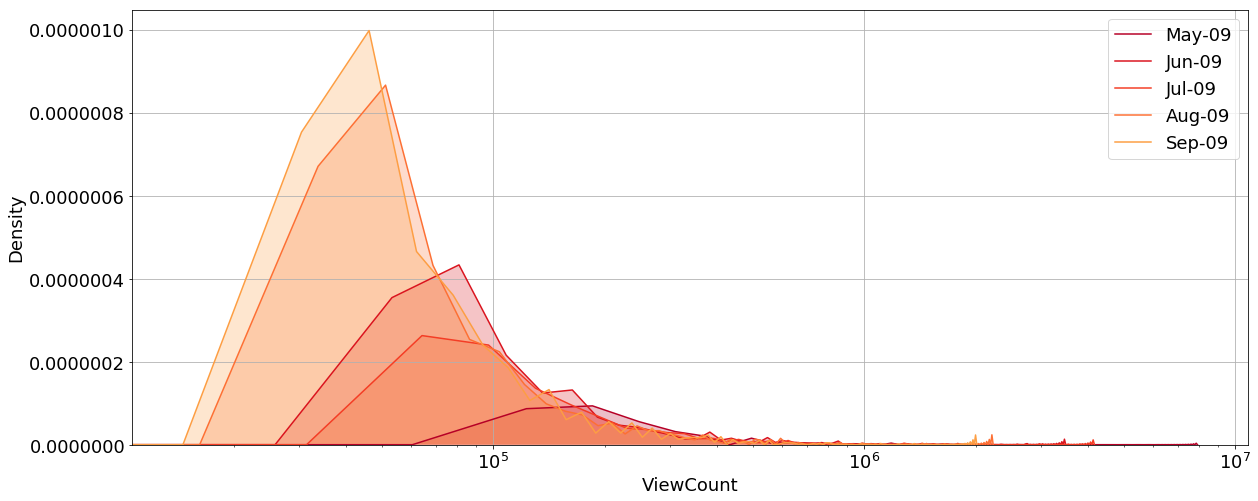
\includegraphics[width=1\linewidth]{../../01-python-code/00-workspace/01-eda/01-graphs/viewcount-sgl-density-plot} \end{center}
\centering {\footnotesize Source: Own calculations in PySpark.}
\end{figure}

\normalsize

\footnotesize

\begin{figure}
\caption{\textbf{Score Density Plot}}
\label{fig:score_dens}

\begin{center}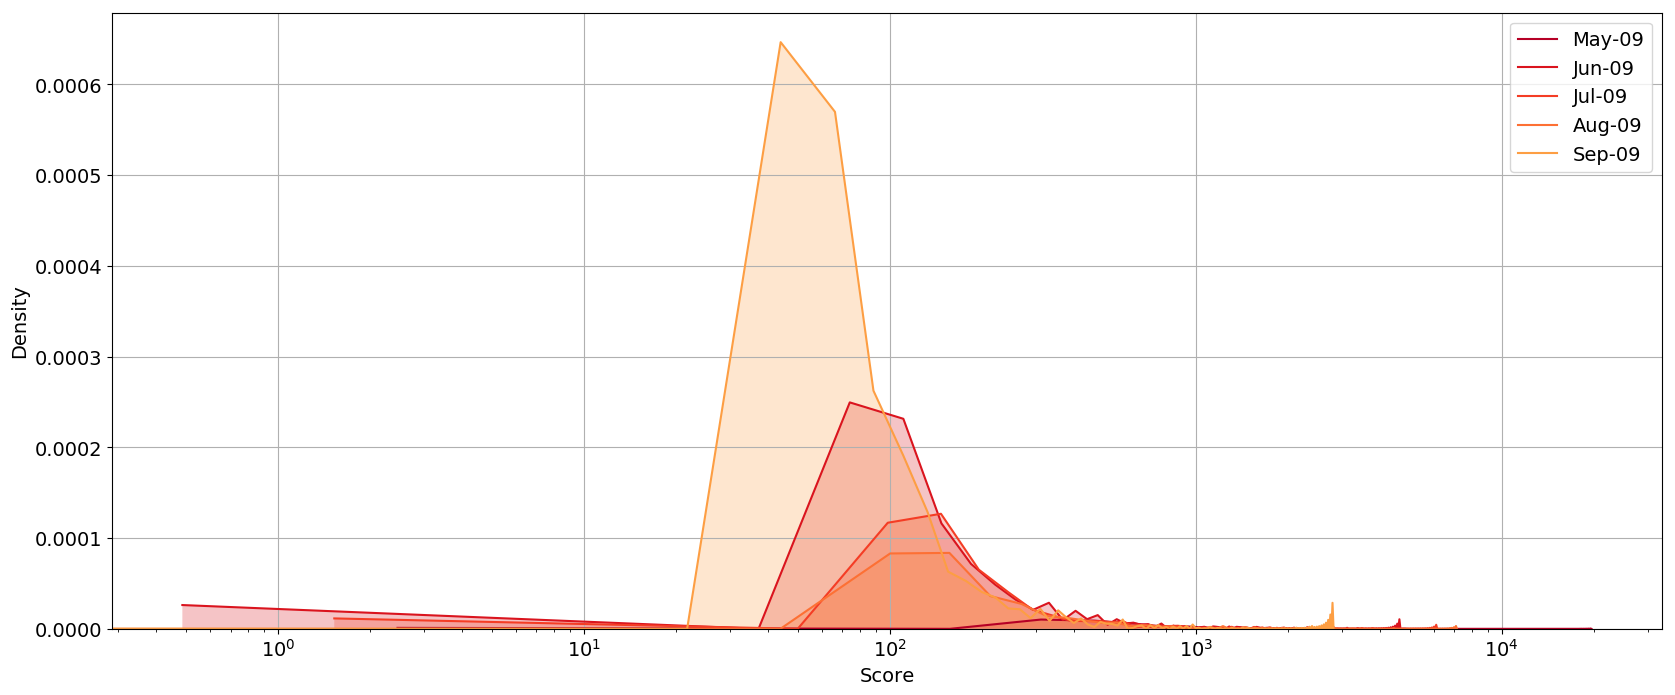
\includegraphics[width=1\linewidth]{../../01-python-code/00-workspace/01-eda/01-graphs/score-sgl-density-plot} \end{center}
\centering {\footnotesize Source: Own calculations in PySpark.}
\end{figure}

\normalsize

As hinted at by table \ref{tab:viewc_desc} and \ref{tab:score_desc}, the
most apparent aspect of the figures above are the differences in
distributions for both the \texttt{Score} and \texttt{ViewCount}
variables. The dataset for May seems to be particularly distinct from
the others for both variables, with substantially flatter and
right-extended distributions.

Despite the differences between distributions, both variables for all
datasets are negatively skewed, \textbf{despite the x-axis already being
log-scaled}. For the \texttt{Score} variable in \ref{fig:score_dens},
the contrasting reputation levels for up- and down-voting privileges (15
and 125 respectively) discussed in the previous section are no doubt a
primary driver of the negative skewness, since it is more likely that
questions will receive an up-vote than a down-vote resulting in more
questions having higher positive \texttt{Scores} and creating the
perception that questions are on average more positively received than
negatively.

\textbf{The explanation} of the negative skewness for the
\texttt{ViewCount} variable in \ref{fig:viewc_dens} seems to stem from
the posts in \textbf{online Q\&A communities} obeying Benford's, Zipf's
and Pareto's laws (see
\url{https://workplace.meta.stackexchange.com/questions/5018/massive-viewcount-difference}).
As evident in the figures above, these laws point to a small subset of
questions being outliers and having high \texttt{ViewCounts} and
\texttt{Scores}, whereas the majority of questions do not. \textbf{This
may complicate modelling}.

\textbf{I now permanently use a logged viewcount variable and a shifted
+ logged score variable}. These variables are plotted below in violin
and boxplots to investigate outliers:

\footnotesize

\begin{figure}
\caption{\textbf{Outlier Plots}}
\label{fig:outlier}
\begin{minipage}{1\textwidth}

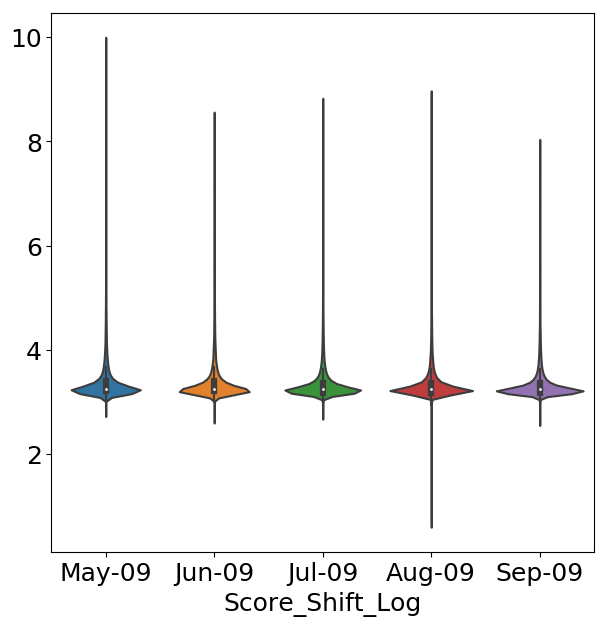
\includegraphics[width=0.49\linewidth]{../../01-python-code/00-workspace/01-eda/01-graphs/score_shift_log-violin-plot} 
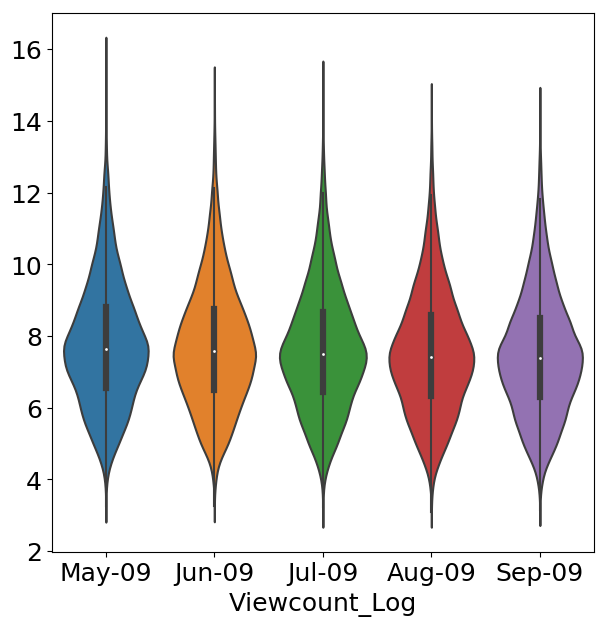
\includegraphics[width=0.49\linewidth]{../../01-python-code/00-workspace/01-eda/01-graphs/viewcount_log-violin-plot} 
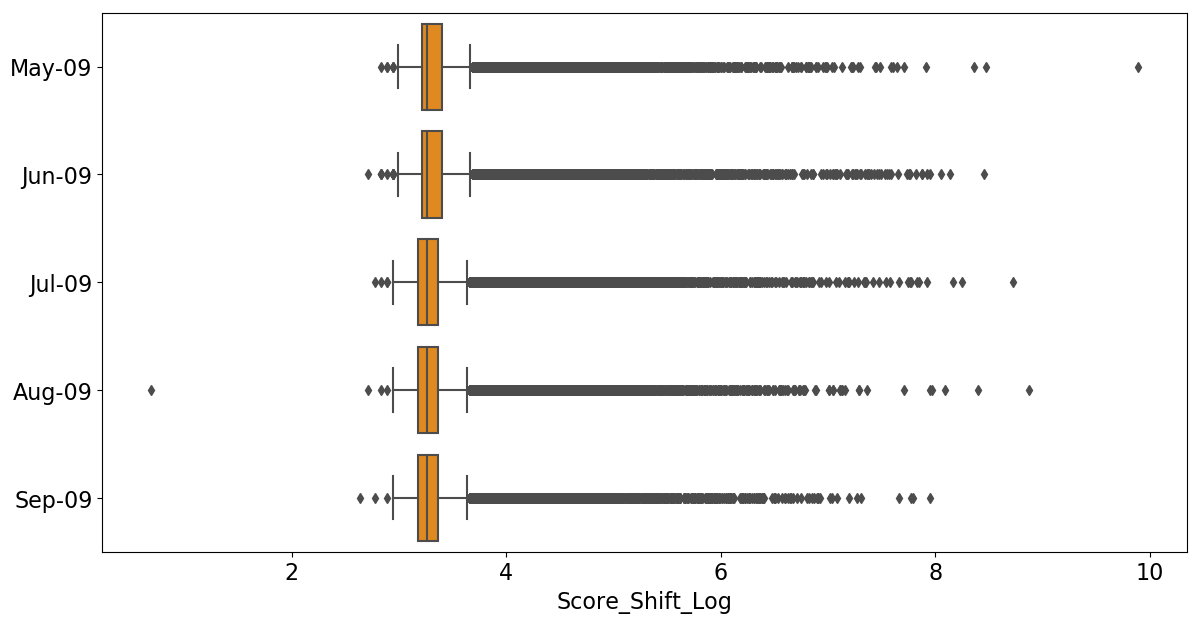
\includegraphics[width=0.49\linewidth]{../../01-python-code/00-workspace/01-eda/01-graphs/score_shift_log-box-plot} 
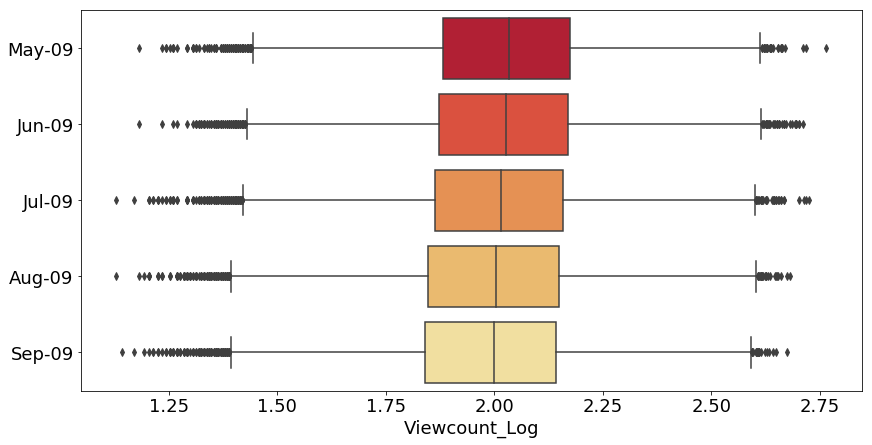
\includegraphics[width=0.49\linewidth]{../../01-python-code/00-workspace/01-eda/01-graphs/viewcount_log-box-plot} 
\\ \centering
{\footnotesize Source: Own calculations in PySpark.}
\end{minipage}
\end{figure}

\normalsize

This brings us to a discussion of what the distinction between the
\texttt{Score} and \texttt{ViewCount} variables actually is. When
looking at the two variables' correlations across datasets in table
\ref{tab:corr} below, it is clear they are both heavily correlated. We
know that more views, and thus a higher \texttt{ViewCount}, implies a
higher \texttt{Score} since owing to unsymmetrical up/down-voting
privileges if a question was to get a vote at all, it is most likely to
get an up-vote, but we don't know how much questions with higher
\texttt{Scores} spur on more views (as the questions rise to the top of
popular search engines etc.), or how much more views spur on more views
for that matter.

\footnotesize

\begin{longtable} {@{} cc @{}}
\caption{\textbf{Score and ViewCount Correlations}}
\label{tab:corr}\\ 
\toprule
\textbf{Dataset} & \textbf{Correlation} \\ 
\midrule
May-09 & 0.86 \\
Jun-09 & 0.85 \\
Jul-09 & 0.81 \\
Aug-09 & 0.71 \\
Sep-09 & 0.76 \\
\bottomrule
\end{longtable}\begin{center} Source: Own calculations in PySpark.\end{center}

\normalsize

Regardless, it is worth noting that only members that have registered
with the community are able to up-vote and down-vote and thus contribute
to the \texttt{Score}, but that fact that all questions are open to the
public implies that the \texttt{ViewCount} variable registers views from
1) registered users that can vote, 2) registered users that can't vote
due to a reputation level below 15, and 3) non-registered members.

Therefore while Ravi \emph{et al.} (2014) considers \texttt{ViewCount}
as a proxy for popularity and consequently in the interest of measuring
question quality divides \texttt{Score} by \texttt{ViewCount} to
mitigate conflating popularity with question quality - I assert that we
have no way of knowing what the composition of the views for a given
question is - i.e.~even though they normalise, are they dividing by
views from people that can't vote or can vote?

I establish a different frame work of \emph{within-community} engagement
versus \emph{outer-community engagement}. With these two definitions in
mind, it is easy to see that the \texttt{Score} variable is primarily a
within-community engagement metric because users are required to commit
and register with a community to contribute to this variable by voting.
\texttt{ViewCount} on the other hand, can be seen as both a within- and
outer- community engagement variable, since it does not distinguish
regarding voting or non-voting status when registering question views.

\textbf{In this vein,} I believe the decision to focus solely on
within-community engagement in my methodology and analysis is robust and
comrephensive, and therefore use the \texttt{Score} variable as it is
rather than normalise by the \texttt{ViewCount} variable. While
popularity, or outer-community engagement, still may influence this
variable to some extent as views drive more registered users to the
question who subsequently vote, I take it as given that having the
ability to attract views is yet another facet of attracting positive
community engagement. It should lastly be noted that questioners would
be more interested in seeing their final \texttt{Score} prediction
rather than \texttt{ViewCount} or \texttt{Score}/\texttt{ViewCount}.

Finally, table \ref{tab:bestworst} displays the titles and details of
StackOverflow questions with the highest and lowest \texttt{Scores} per
dataset.

\footnotesize

\begin{longtable} {@{} cccp{11cm} @{}}
\caption{\textbf{Highest and Lowest Scored Questions Across Datasets}}
\label{tab:bestworst}\\ 
\toprule
\textbf{Dataset} & \textbf{Score} & \textbf{ViewCount} & \textbf{Title} \\ 
\midrule
May-09 &  19640 &    7906137 &  How do I undo the most recent local commits in Git? \\
May-09 &     -7 &        792 &                       List Element without iteration \\
Jun-09 &   4655 &    2729671 &                            How do I include a JavaScript file in another JavaScript file? \\
Jun-09 &     -9 &       1664 &  How can I use a class from a header file in a source file using extern but not \#include? \\
Jul-09 &   6145 &    3792462 &    How do I force "git pull" to overwrite local files? \\
Jul-09 &     -8 &        349 &  Why does this C function not return an integer value? \\
Aug-09 &   7133 &    1018228 &  What does "use strict" do in JavaScript, and what is the reasoning behind it? \\
Aug-09 &    -22 &        934 &                                      Getting Row from Gridview in Dev Express? \\
Sep-09 &   2809 &     559244 &  Move existing, uncommitted work to a new branch in Git \\
Sep-09 &    -10 &        362 &        Which object is created in which part of memory? \\
\bottomrule
\end{longtable}\begin{center} Source: Own calculations in PySpark.\end{center}

\normalsize

By using just the \texttt{Score} variable in my methodology as a
response variable, the above questions show that \textbf{everything
works.}

\subsubsection{\texorpdfstring{Potential Methodological Issues
\label{Issues}}{Potential Methodological Issues }}\label{potential-methodological-issues}

Regarding confounding issues for the \texttt{Score} variable, it is
worth remembering that questions can be edited, not only by the original
poster, but by anyone with a level of reputation of 2~000 or more.
General cross-community guidelines for editing include addressing
grammar and spelling issues, clarifying concepts, correcting minor
mistakes, and adding related resources and links. The concern here is
that users could vote, comment and answer on substantially different
questions over time as a question is edited further away from it's
original form. The simplifying assumption that I make here is that most
edits, if any at all, happen quickly as moderators and high-reputation
users are made aware of offending questions and thus the majority of
views and votes would happen on final, edited questions. I therefore
choose to analyse the final edited question content.

Another factor is community behaviour confusion - there seems to be a
less-than-full consensus of when exactly to up- or down-vote (see
\url{https://meta.stackexchange.com/questions/12772/should-i-upvote-bad-questions})
despite general guidelines on StackExchange sites stating that up-votes
should be given if a question shows prior research, is clear and useful,
and down-voting the opposite. I assume that this confusion is small and
evenly distributed over the data.

A second methodological adjustment that Ravi \emph{et al.} (2014) make
with their data is to only consider questions above a certain minimum
\texttt{ViewCount} threshold. Their reasoning behind this is to increase
their confidence that the final dataset contains questions that have
been viewed by qualifying users that can vote. Again, we do not know if
views are from people that can or can't vote, so assuming is wrong. I
believe this is a false claim, since one could just as easily argue that
new questions that begin with a low \texttt{ViewCount} are more likely
to see engagement from \emph{proactive} community members, especially if
these questions don't generate enough webpage activity to rise as the
top hit for search engines (which would lead to more non-community
member activity contribution to views). Since there is also no data on
the distribution of qualifying and non-qualifying user contributions to
the \texttt{ViewCount} variable, I opt to \emph{not} disregard any
questions below a certain \texttt{ViewCount} threshold.

\newpage

\subsection{\texorpdfstring{Model \label{Model}}{Model }}\label{model}

\subsubsection{Elastic-net Regularised Regression
Model}\label{elastic-net-regularised-regression-model}

Let \(q_i\) denote question \(i\) out of all questions \(Q\) with score
\(s_i\). I use elastic-net regularised regression to predict \(s_i\) for
each question using only features derived from the raw textual
\texttt{Body} and \texttt{Title} independent variables, which I denote
\(\bm{x'}_i\). A choice now needs to be made between using the
root-mean-square error (RMSE) or the mean-absolute error (MAE) to
evaluate and compare models.

({\textbf{???}}) investigate the aversion to use RMSE in the literature
in more detail. Contrary to prior work advocating for the avoidance of
RMSE, they note that RMSE is the more appropriate metric when the error
distribution of the model is expected to be Gaussian instead of uniform
and RMSE gives more weight to outliers, therefore penalising variance.
It should also be noted, that by definition, RMSE can never be smaller
than MAE.

The learning objective can therefore be summarised as finding a
coefficient vector \(\bm{\beta}\) which minimises the chosen metric:

\begin{align} \label{eq:rmse}
\underset{\bm{\beta}}{\text{minimise}} \quad \sqrt{ \frac{1}{|Q_\text{train}|} \sum_{ q_{i} \in Q_{\text{train}} } ( s_i - {\bm{\beta}\bm{x'}_i} )^2 + \Psi }
\end{align}

where

\begin{align} \label{eq:penalty}
\Psi = \lambda \sum_{j=1}^p ( \alpha\beta_j^2 + (1-\alpha)|\beta_j| )
\end{align}

is the elastic net penalty term. \textbf{WHY CHOSE RMSE AS METRIC}

In this term, \(\lambda\) is the regularisation parameter for the
prevention of over-fitting, \(\alpha\) is a weighting coefficient for
the \(L_1\) and \(L_2\) norms of the input variables, corresponding to
the lasso and ridge penalties for \(\alpha=1\) and \(\alpha=0\)
respectively. \textbf{MORE}

\textbf{LASSO better when there are variables that are useless (they get
shrunken to 0), RIDGE better when all are useful because it will shrink
parameters but not eliminate.}

\subsubsection{Train/Test Split}\label{traintest-split}

I split the datasets into a training set \(Q_\text{train}\) (50\%) and a
testing set \(Q_\text{test}\) (50\%). I choose a 50/50 train/test split
because I believe that the size of the datasets allows for enough
training data, and this decision coincides with the train/test split of
Ravi \emph{et al.} (2014). The standard deviations of a random splitting
of training and testing sets is displayed in table \ref{tab:rand_tr_te}
below.

\textbf{Use SD or \(\sigma\)?}

\footnotesize

\begin{longtable}[htbp] {@{} lccc @{}} 
\caption{\textbf{Random Train/Test Split Standard Deviations}} 
\label{tab:rand_tr_te} \\
\toprule
\textbf{Dataset} &  \textbf{Train SD} &  \textbf{Test SD} & \textbf{\% Difference} \\
\midrule
May-09 & 186 & 75 & -60 \\
Jun-09 & 73 & 99 & 36 \\
Jul-09 & 62 & 89 & 44 \\
Aug-09 & 82 & 57 & -30 \\
Sep-09 & 50 & 45 & -10 \\
\bottomrule
\end{longtable}\begin{center} Source: Own calculations in PySpark\end{center}

\normalsize

We see in table \ref{tab:rand_tr_te} that the standard deviations are
\ldots{}

However, just to be sure we also split the training and testing data
temporally within each of the eight datasets to cautiously test my
assumption of homogeneity with regard to time within each dataset. These
standard deviations are shown in table \ref{tab:time_tr_te}.

\footnotesize

\begin{longtable}[htbp] {@{} lccc @{}} 
\caption{\textbf{Temporal Train/Test Split Standard Deviations}} 
\label{tab:time_tr_te} \\
\toprule
\textbf{Dataset} &  \textbf{Train SD} &  \textbf{Test SD} & \textbf{\% Difference} \\
\midrule
May-09 & 72 & 188 & 161 \\
Jun-09 & 89 & 85 & -4 \\
Jul-09 & 87 & 64 & -26 \\
Aug-09 & 63 & 78 & 24 \\
Sep-09 & 47 & 47 & 0 \\
\bottomrule
\end{longtable}\begin{center} Source: Own calculations in PySpark\end{center}

\normalsize

This shows that the data is \textbf{HOPEFULLY NOT} heterogenous with
regard to time, supporting my hypothesis that the datasets do not
exhibit temporal trends due to how the communities have evolved over
time or how questions have evolved.

I thus use the random train/test split for \textbf{my entire analysis}.

I use 2-fold cross validation - 2 because increasing the number of folds
did not lead to large gains in RMSE reduction over models in general,
and also drastically increased computation time.

\subsubsection{Question Content}\label{question-content}

A number of preprocessing steps are applied to the \texttt{Body} and
\texttt{Title} to obtain the final features \(\bm{x'}_i\) that are
discussed subsequently - I parsed the HTML of the question content in
the \texttt{Body} variable, tokenised (with punctuation) both the
\texttt{Body} and \texttt{Title} texts, removed English stopwords and
stemmed tokens using Porter-stemming ({\textbf{???}}).

I first extract features relating to the length of questions'
\texttt{Body} and \texttt{Title}, i.e.~token count, sentence count and
character count. Then, the actual unigram text of the question
\texttt{Body} and \texttt{Title} are used as features in the form of
term frequency -- inverse document frequencies (TF-IDF). \textbf{MORE}
\textbf{Since Ravi \emph{et al.} (2014) do not use higher order ngrams,
I also stick to unigrams, resulting in quick and compact learning.}

\subsubsection{Topic Modelling}\label{topic-modelling}

I train an LDA model globally over all questions in \(Q\). I use the
online LDA learning framework in the Pyspark \texttt{pyspark.sql.ml}
package to generate topic distributions over words for each question as
a global LDA model, and over sentences as a local LDA model and add
these as model features. This results in features made up of weights
\(\theta_{qt}\) for a topic \(t\) in a question \(q\), and with
\(\theta_{qt}=P(t|q).\)

I choose \(K=10\) topics

\textbf{Online LDA works like this}

\subsection{EXTRA}\label{extra}

This touches on a point that was not considered in Ravi \emph{et al.}
(2014) nor in previous research to my knowledge - the temporal nature of
online Q\&A questions. I believe that predicting \texttt{Scores} of
future questions may prove a substantially more difficult task than just
randomising the training and testing question sets.

Note however that not included a temporal element to my model, so if
there are some time-series trends in the data (to do with the struture
of the websites changing etc.), then the temporal prediction will be
poor.

\textbf{Since this analysis has already taken the first step from prior
research to look more broadly at community engagement, and a continuous
response in addition, potential temporality of the data will not be
thoroughly explored in the form of implementation of time-series models,
but will be touched on by comparing model results for a random
train/test split versus chronological.}

\newpage

\section{\texorpdfstring{Results
\label{Results}}{Results }}\label{results}

To establish a baseline for the predictive performance of the models,
table \ref{tab:rand_mean_model} displays training and testing RMSE
values across datasets for a model that predicts the constant mean of
the training set for every question in the testing set.

\footnotesize

\begin{longtable}[htbp] {@{} lccc @{}} 
\caption{\textbf{Constant Mean Model}} 
\label{tab:rand_mean_model} \\
\toprule
\textbf{Dataset} &  \textbf{Train RMSE} &  \textbf{Test RMSE} &  \textbf{Time (s)} \\
\midrule
May-09 &                185.85 &              75.37 &                 1  \\
Jun-09 &                 89.59 &              84.77 &                 1  \\
Jul-09 &                 85.21 &              66.81 &                 1  \\
Aug-09 &                 83.27 &              55.47 &                 1  \\
Sep-09 &                 42.76 &              51.12 &                 1  \\
\bottomrule
\end{longtable}\begin{center} Source: Own calculations in PySpark\end{center}

\normalsize

The values in the Test RMSE column in table \ref{tab:rand_mean_model}
are considered the low benchmarks that future models must improve upon.
A few aspects area worthing noting in table \ref{tab:rand_mean_model}
alone. Firstly, we see that the test RMSE is lower than train RMSE for
both May and August. Secondly, the difference for May is stark, with the
test RMSE being less than half the train RMSE. This nois in spite of a
random splitting of train and test sets, and is evidence of the sheer
amount of variation (and probably noise) in the data.

Looking back at \ref{tab:tab:score_desc}, we see that May was the
dataset with the largest standard deviation for the \texttt{Score}
variable. The RMSE is different per community owing to the different
standard deviations of the data as a whole seen in the EDA.

\footnotesize

\begin{longtable}[htbp] {@{} lcccc @{}} 
\caption{\textbf{ViewCount Model}} 
\label{tab:rand_view_model} \\
\toprule
\textbf{Dataset} &  \textbf{Train RMSE} &  \textbf{Test RMSE} &  \textbf{Test Gain (\%)} &  \textbf{Time (s)} \\
\midrule
May-09 &                81.03 &             75.01 &               0.48 &               11 \\
Jun-09 &                49.68 &             43.05 &              49.22 &                7 \\
Jul-09 &                48.43 &             41.96 &              37.20 &                7 \\
Aug-09 &                61.35 &             36.99 &              33.32 &                7 \\
Sep-09 &                23.56 &             36.39 &              28.81 &                7 \\
\bottomrule
\end{longtable}\begin{center} Source: Own calculations in PySpark\end{center}

\normalsize

Table \ref{tab:rand_view_model} above is the high benchmark owing to the
strong correlations seen in table \ref{tab:corr} and the fact that it is
measuring essentially both within-community engagement and
outer-community engagement. Column Test Gain shows the percentage
improvement over the test RMSE of the low benchmark models. If any of
the models come close to achieving these improvements, it would be
great. It should obviously be noted that this model is vacuous, since
the final \texttt{ViewCount} of a question is not available for new
questions.

\footnotesize

\begin{longtable}[htbp] {@{} lcccccc @{}} 
\caption{\textbf{Length Model}} 
\label{tab:rand_count_model} \\
\toprule
\textbf{Dataset} &  \textbf{Train RMSE} &  \textbf{Test RMSE} &  \textbf{Test Gain (\%)} & \textbf{$\lambda$} & \textbf{$\alpha$} &  \textbf{Time (s)} \\
\midrule
May-09 &            185.80 &          75.35 &            0.03 &               1 &              0.01 &            13 \\
Jun-09 &             89.53 &          84.71 &            0.07 &               1 &              1 &            12 \\
Jul-09 &             85.15 &          66.76 &            0.07 &               1 &              1 &            16 \\
Aug-09 &             83.25 &          55.43 &            0.07 &               1 &              1 &            14 \\
Sep-09 &             42.71 &          51.06 &            0.12 &               1 &              0.01 &            12 \\
\bottomrule
\end{longtable}\begin{center} Source: Own calculations in PySpark\end{center}

\normalsize

Table \ref{tab:rand_count_model} shows minuscle improvements over the
constant mean benchmark, with approximately 0.06\% improvements in RMSE
depicted in the Test Gain column. There are also almost barely any
improvements across the train RMSE. We see that the best models selected
by the grid search all had a regularisation parameter of 1, implying
that full regularisation was employed, but the May and September
datasets stand out as the only models where \textbf{ridge} was selected
(alpha=0.01) where a selection of parameters were not entirely shrunk to
0.

\footnotesize

\begin{longtable}[htbp] {@{} lcccccc @{}} 
\caption{\textbf{Unigram Textual Model}} 
\label{tab:rand_token_model} \\
\toprule
\textbf{Dataset} &  \textbf{Train RMSE} &  \textbf{Test RMSE} &  \textbf{Test Gain (\%)} & \textbf{$\lambda$} & \textbf{$\alpha$} &  \textbf{Time (s)} \\
\midrule
May-09 &             96.65 &         299.68 &         -297.61 &               1 &              1 &          1359.0 \\
Jun-09 &             61.96 &         123.07 &          -45.18 &               1 &              1 &          1736.0 \\
Jul-09 &             21.55 &         208.94 &         -212.74 &               1 &              0.01 &          1793.0 \\
Aug-09 &             34.47 &          98.17 &          -76.98 &               1 &              1 &          1981.0 \\
Sep-09 &             30.67 &          58.73 &          -14.89 &               1 &              1 &          2106.0 \\
\bottomrule
\end{longtable}\begin{center} Source: Own calculations in PySpark\end{center}

\normalsize

The results of using unigram text of question titles and bodies is
displayed in table \ref{tab:rand_token_model}. This model struggles
particularly, evidently overfitting on the training set to obtain
extremely low train RMSE values across models, but hopelessly
underperforming on the test set with RMSEs rocketing up to as high as
552.

Interestingly, the grid search gives an elastic parameter of 1 and
regularisation parameter of 1 for all models except for July.

\footnotesize

\begin{longtable}[htbp] {@{} lcccccc @{}} 
\caption{\textbf{Global and Local Topic Model}} 
\label{tab:rand_topic_model} \\
\toprule
\textbf{Dataset} &  \textbf{Train RMSE} &  \textbf{Test RMSE} &  \textbf{Test Gain (\%)} & \textbf{$\lambda$} & \textbf{$\alpha$} &  \textbf{Time (s)} \\
\midrule
May-09 &            185.62 &          75.75 &           -0.50 &               1 &               1 &            13 \\
Jun-09 &             89.50 &          84.67 &            0.12 &               1 &               1 &            11 \\
Jul-09 &             85.13 &          66.78 &            0.04 &               1 &               1 &            13 \\
Aug-09 &             83.26 &          55.48 &           -0.02 &               1 &               1 &            12 \\
Sep-09 &             42.74 &          51.09 &            0.06 &               1 &               1 &            12 \\
\bottomrule
\end{longtable}\begin{center} Source: Own calculations in PySpark\end{center}

\normalsize

What we have garnered is that the \textbf{datasets are very
heterogenous}, having seen large differences in both the descriptive
statistics and predictive results - different parameters come out as
optimal for the length and topic models.

\footnotesize

\begin{longtable}[htbp] {@{} lcccccc @{}} 
\caption{\textbf{Length and Topic Model}} 
\label{tab:rand_final_model} \\
\toprule
\textbf{Dataset} &  \textbf{Train RMSE} &  \textbf{Test RMSE} &  \textbf{Test Gain (\%)} & \textbf{$\lambda$} & \textbf{$\alpha$} &  \textbf{Time (s)} \\
\midrule
May-09 &           185.58 &         75.72 &          -0.46 &              1 &              1 &           14 \\
Jun-09 &            89.43 &         84.60 &           0.20 &              1 &              1 &           12 \\
Jul-09 &            85.06 &         66.73 &           0.12 &              1 &              1 &           14 \\
Aug-09 &            83.24 &         55.44 &           0.05 &              1 &              1 &           14 \\
Sep-09 &            42.71 &         51.06 &           0.12 &              1 &              1 &           17 \\
\bottomrule
\end{longtable}\begin{center} Source: Own calculations in PySpark\end{center}

\normalsize

\textbf{Temporal Train/Test Split}

\footnotesize

\begin{longtable}[htbp] {@{} lcccccc @{}} 
\caption{\textbf{Length and Topic Model For Temporal Train/Test Split}} 
\label{tab:time_token_model} \\
\toprule
\textbf{Dataset} &  \textbf{Train RMSE} &  \textbf{Test RMSE} &  \textbf{Test Gain (\%)} & \textbf{$\lambda$} & \textbf{$\alpha$} &  \textbf{Time (s)} \\
\midrule
May-09 &            71.65 &        187.57 &        -148.87 &              1.0 &             1.00 &           20.0 \\
Jun-09 &            88.74 &         85.34 &          -0.67 &              1.0 &             1.00 &           12.0 \\
Jul-09 &            87.05 &         64.26 &           3.82 &              1.0 &             1.00 &           13.0 \\
Aug-09 &            62.62 &         78.07 &         -40.74 &              1.0 &             1.00 &           13.0 \\
Sep-09 &            47.18 &         46.76 &           8.53 &              1.0 &             0.01 &           15.0 \\
\bottomrule
\end{longtable}\begin{center} Source: Own calculations in PySpark\end{center}

\normalsize

\newpage

\section{\texorpdfstring{Recommendations for Further Research
\label{Recom}}{Recommendations for Further Research }}\label{recommendations-for-further-research}

A number of areas for further research stand out from the methodology I
developed here. Firstly, there are still many more complex features that
can be derived from question content alone that were not included in the
models in this research. Word-embeddings (({\textbf{???}})) might be
\textbf{more} successful in predicting community engagement metrics.

As discussed \textbf{in detail} in section \ref{Vars}, there are also a
myriad of other options for community engagement besides the
\texttt{Score} variable, each with their own advantages and
disadvantages. While I believe I thoroughly justified and validated my
choice of the continuous \texttt{Score} variable as a comprehensive and
objective response variable, not least because accurate predictions of
it would be \textbf{highly useful information for questioners wishing to
improve their questions}, a thorough exploration and predictive modeling
of other measurements of community engagement with the models developing
here would be extremely valuable.

Another area previously discussed that is ripe for further research is
the editing of questions. As a reminder, questions can be edited not
only by the original poster, but also by anyone with \textbf{2000}
reputation or more. One suggestion for further research would be
investigating how much editing takes place over questions, in what
average timeframe edits are completed compared to votes cast and views
accumulated, as well as how evenly editing is distributed over
questions. This research would then be able to test my assumption that
most edits, if any, take place before the majority of votes and views
are recorded.

There are also finer nuances regarding the functioning of the
StackExchange sites, \textbf{some of which were} discussed in section
\ref{Issues}. For registered users in various communities, there remains
some confusion on when to up-vote and down-vote questions (see
\url{https://meta.stackexchange.com/questions/12772/should-i-upvote-bad-questions}).
This links with how there are potentially vastly different motivations
behind voting? Over time various communities have also implemented
different interventions to nudge users to better formulate and structure
their questions, i.e.~reminders of doing prior research, including
reproducible code for programming websites, and even going as far as to
check that the \texttt{Title} of new questions do not match previous
questions too closely for fear of allowing a duplicate question to be
asked in the community. These nudges would no doubt affect the
distribution and evolution of questions temporally in the data, and
consequently affect metrics such as \texttt{Score} and
\texttt{ViewCount}, which links with the next final recommendation for
further research.

\textbf{Most} importantly as hinted throughout and demonstrated at the
end of this analysis, temporality of the data is something that needs to
be taken into account. This is at least true in the sense that questions
which have existed longer in communities trivially would have had more
time to accumulate votes and views, but my further hypothesis is that
the variation in community engagement metrics has decreased
substantially over time as users and communities have refined how they
permit and value certain questions - this new hypothesis of
heterogeneity over time can be tested with variance equivalence testing
for samples across time. All of this suggests that any model aiming to
predict future community engagement in online Q\&A fora must be expanded
to include temporal effects and time-series elements.

Even if the temporality issue was solved however, another challenge is
getting the model to pick up duplicate questions (which are
ill-considered in all communities). This would mean instilling in the
model that a question can be similar enough to previous questions for
the model to learn that it's a good question, however not too similar so
that the community perceives it as a duplicate, assumes a ``lack of
prior research'' on the questioner's part and then reacts negatively to
the question. As one can see therefore, there is still much work to be
done in order to accurately predict future communtity engagement in
online Q\&A fora.

\textbf{I also find that models across fora have varying} levels of
performance, \textbf{providing evidence} against claims in Ravi \emph{et
al.} (2014) that topic models are applicable to different online Q\&A
settings. While comparison across fora is limited owing to differences
in community age, daily traffic, number of users etc\ldots{} . Ravi
\emph{et al.} (2014) specifically state that ``{[}their{]} methods do
not rely on domain-specific knowledge'' and therefore ``{[}they{]}
believe {[}the methods{]} are applicable to other CQA settings as
well''. I believe that community behavior is too diverse to be
universally predicted by a single model, thus I will begin to gain some
insight into whether the predictive model I build works as effectively
across all the communities I analyse.

\subsection{EXTRA}\label{extra-1}

While I do not employ time-series models, I leave it to further research
to incorporate a way to also ``remember'' which questions are good, so
that in future there are no duplicates.

\textbf{EVEN AFTER GETTING RID OF A SUBSTANTIAL AMOUNT OF DATA FOR
CERTAIN DATASETS BY USING ONLY A YEAR WORTH OF DATA in the early stages
of the communitites' existence, THE TEMPORAL MODEL STILL STRUGGLES
SUBSTANTIALLY.}

\newpage

\section{\texorpdfstring{Concluding Remarks
\label{Concl}}{Concluding Remarks }}\label{concluding-remarks}

The aim of this research was to predict the range of positive/negative
community engagement that questions elicit, with the practical
application of providing this information to questioners so that they
can improve their questions before adding demand to a community. I
believe that no prior research has endeavoured with the methodology here
in this respective framework to predict and capture community
engagement. At the very least, the research here has improved upon the
extent of how community engagement can be ascertained from online Q\&A
communities, and has yielded insight into how homogeneously community
engagement exists over diverse communities with various subject matter.
I believe that using this tool, online Q\&A users will be assisted in
improving their submitted questions which will enhance the productivity
of all online Q\&A communities wholly. Furthermore, room exists for
implementation on any assortment of Q\&A sites, counting Massive Open
Online Courses.

\textbf{There is much heterogeneity in the data I have analysed with
regard to time. This, as well as the fact that I have attempted to
predict on a continuous variable rather than binary, makes the problem
of predicting community engagement from text-only data substantially
more difficult, as can be seen from the poor predictive performance of
the models employed. I leave it to future research to employ more
sophisticated time-series models to capture temporal effects/features
from the data.}

\newpage

\section*{References}

\hypertarget{refs}{}
\hypertarget{ref-Agichtein2008}{}
Agichtein, E. \emph{et al.} (2008) `Finding high-quality content in
social media', in \emph{Proceedings of the 2008 international conference
on web search and data mining}. ACM, pp. 183--194. doi:
\href{https://doi.org/10.1145/1341531.1341557}{10.1145/1341531.1341557}.

\hypertarget{ref-Allamanis2013}{}
Allamanis, M. and Sutton, C. (2013) `Why, when, and what: Analyzing
stack overflow questions by topic, type, and code', in \emph{2013 10th
working conference on mining software repositories (msr)}. IEEE, pp.
53--56. doi:
\href{https://doi.org/10.1109/MSR.2013.6624004}{10.1109/MSR.2013.6624004}.

\hypertarget{ref-Anderson2012}{}
Anderson, A. \emph{et al.} (2012) `Discovering value from community
activity on focused question answering sites: a case study of stack
overflow', in \emph{Proceedings of the 18th acm sigkdd international
conference on knowledge discovery and data mining}. ACM, pp. 850--858.
Available at: \url{http://dl.acm.org/citation.cfm?id=2339665}.

\hypertarget{ref-Bian2009}{}
Bian, J. \emph{et al.} (2009) `Learning to recognize reliable users and
content in social media with coupled mutual reinforcement', in
\emph{Proceedings of the 18th international conference on world wide
web}. ACM, pp. 51--60. doi:
\href{https://doi.org/10.1145/1526709.1526717}{10.1145/1526709.1526717}.

\hypertarget{ref-Blei2003}{}
Blei, D. M., Ng, A. Y. and Jordan, M. I. (2003) `Latent Dirichlet
Allocation', \emph{Journal of Machine Learning Research}, 3, pp.
993--1022.

\hypertarget{ref-Chiang2010}{}
Chiang, D. \emph{et al.} (2010) `Bayesian Inference for Finite-State
Transducers', in \emph{Human language technologies: The 2010 annual
conference of the north american chapter of the association for
computational linguistics}. Association for Computational Linguistics
(June), pp. 447--455. Available at:
\href{http://www.isi.edu/\%7B~\%7Dsravi/pubs/naacl2010\%7B/_\%7Dbayes-fst.pdf}{http://www.isi.edu/\{\textasciitilde{}\}sravi/pubs/naacl2010\{\textbackslash{}\_\}bayes-fst.pdf}.

\hypertarget{ref-Daume2006}{}
Daumé, H. and Marcu, D. (2006) `Bayesian query-focused summarization',
\emph{COLING/ACL 2006 - 21st International Conference on Computational
Linguistics and 44th Annual Meeting of the Association for Computational
Linguistics, Proceedings of the Conference}, 1, pp. 305--312.

\hypertarget{ref-Eppler2004}{}
Eppler, M. J. and Mengis, J. (2004) `The concept of information
overload: A review of literature from organization science, accounting,
marketing, MIS, and related disciplines', \emph{Information Society},
20(5), pp. 325--344. doi:
\href{https://doi.org/10.1080/01972240490507974}{10.1080/01972240490507974}.

\hypertarget{ref-Fligner1986}{}
Fligner, M. and Verducci, J. S. (1986) `Distance based ranking models',
\emph{Journal of the Royal Statistical Society: Series B
(Methodological)}, 48(3), pp. 359--369.

\hypertarget{ref-Haghighi2010}{}
Haghighi, A. and Klein, D. (2010) `Coreference Resolution in a Modular,
Entity-Centered Model', (June), pp. 385--393.

\hypertarget{ref-Jeon2006}{}
Jeon, J. \emph{et al.} (2006) `A framework to predict the quality of
answers with non-textual features', in \emph{Proceedings of the 29th
annual international acm sigir conference on research and development in
information retrieval}. ACM, pp. 228--235. doi:
\href{https://doi.org/10.1145/1148170.1148212}{10.1145/1148170.1148212}.

\hypertarget{ref-Kozareva2011}{}
Kozareva, Z. and Ravi, S. (2011) `Unsupervised name ambiguity resolution
using a generative model', \emph{\ldots{} First Workshop on Unsupervised
Learning in NLP}, pp. 105--112. Available at:
\url{http://dl.acm.org/citation.cfm?id=2140471}.

\hypertarget{ref-Li2010}{}
Li, B. and King, I. (2010) `Routing questions to appropriate answerers
in community question answering services', in \emph{Proceedings of the
19th acm international conference on information and knowledge
management}. ACM, pp. 1585--1588. doi:
\href{https://doi.org/10.1145/1871437.1871678}{10.1145/1871437.1871678}.

\hypertarget{ref-Li2012}{}
Li, B. \emph{et al.} (2012) `Analyzing and predicting question quality
in community question answering services', in \emph{Proceedings of the
21st international conference on world wide web}. ACM, pp. 775--782.
doi:
\href{https://doi.org/10.1145/2187980.2188200}{10.1145/2187980.2188200}.

\hypertarget{ref-Li2011}{}
Li, B., King, I. and Lyu, M. R. (2011) `Question routing in community
question answering', in \emph{Proceedings of the 20th acm international
conference on information and knowledge management}. ACM, pp.
2041--2044. doi:
\href{https://doi.org/10.1145/2063576.2063885}{10.1145/2063576.2063885}.

\hypertarget{ref-Liu2008}{}
Liu, Y., Bian, J. and Agichtein, E. (2008) `Predicting information
seeker satisfaction in community question answering', in
\emph{Proceedings of the 31st annual international acm sigir conference
on research and development in information retrieval}. ACM (Section 2),
pp. 483--490. doi:
\href{https://doi.org/10.1145/1390334.1390417}{10.1145/1390334.1390417}.

\hypertarget{ref-Qu2009}{}
Qu, M. \emph{et al.} (2009) `Probabilistic question recommendation for
question answering communities', in \emph{Proceedings of the 18th
international conference on world wide web}. ACM (2), pp. 1229--1230.
doi:
\href{https://doi.org/10.1145/1526709.1526942}{10.1145/1526709.1526942}.

\hypertarget{ref-Ravi2014}{}
Ravi, S. \emph{et al.} (2014) `Great Question! Question Quality in
Community Q\&A.', in \emph{Eighth international aaai conference on
weblogs and social media}. (1), pp. 426--435.

\hypertarget{ref-Reisinger2009}{}
Reisinger, J. and Paşca, M. (2009) `Latent variable models of
concept-attribute attachment', (August), p. 620. doi:
\href{https://doi.org/10.3115/1690219.1690233}{10.3115/1690219.1690233}.

\hypertarget{ref-Riahi2012}{}
Riahi, F. \emph{et al.} (2012) `Finding expert users in community
question answering', in \emph{Proceedings of the 21st international
conference on world wide web}. ACM, pp. 791--798. doi:
\href{https://doi.org/10.1145/2187980.2188202}{10.1145/2187980.2188202}.

\hypertarget{ref-Ritter2010}{}
Ritter, A., Mausam and Etzioni, O. (2010) `A latent dirichlet allocation
method for selectional preferences', \emph{ACL 2010 - 48th Annual
Meeting of the Association for Computational Linguistics, Proceedings of
the Conference}, (July), pp. 424--434.

\hypertarget{ref-Shah2010}{}
Shah, C. and Pomerantz, J. (2010) `Evaluating and predicting answer
quality in community QA', in \emph{Proceedings of the 33rd international
acm sigir conference on research and development in information
retrieval}. ACM (March 2008), pp. 411--418. doi:
\href{https://doi.org/10.1145/1835449.1835518}{10.1145/1835449.1835518}.

\hypertarget{ref-Shah2018}{}
Shah, V. \emph{et al.} (2018) `Adaptive matching for expert systems with
uncertain task types', \emph{55th Annual Allerton Conference on
Communication, Control, and Computing, Allerton 2017}, 2018-January, pp.
753--760. doi:
\href{https://doi.org/10.1109/ALLERTON.2017.8262814}{10.1109/ALLERTON.2017.8262814}.

\hypertarget{ref-Sung2013}{}
Sung, J., Lee, J.-g. and Lee, U. (2013) `Booming Up the Long Tails:
Discovering Potentially Contributive Users in Community-Based Question
Answering Services', in \emph{Seventh international aaai conference on
weblogs and social media}, pp. 602--610.

\hypertarget{ref-Szpektor2013}{}
Szpektor, I., Maarek, Y. and Pelleg, D. (2013) `When relevance is not
enough: promoting diversity and freshness in personalized question
recommendation', in \emph{Proceedings of the 22nd international
conference on world wide web}. ACM, pp. 1249--1260.

\hypertarget{ref-Tian2013}{}
Tian, Q., Zhang, P. and Li, B. (2013) `Towards Predicting the Best
Answers in Community-Based Question-Answering Services', in
\emph{Seventh international aaai conference on weblogs and social
media}, pp. 725--728.

\hypertarget{ref-Wu2008}{}
Wu, H., Wang, Y. and Cheng, X. (2008) `Incremental probabilistic latent
semantic analysis for automatic question recommendation', in
\emph{Proceedings of the 2008 acm conference on recommender systems}.
ACM, p. 99. doi:
\href{https://doi.org/10.1145/1454008.1454026}{10.1145/1454008.1454026}.

\hypertarget{ref-Zhou2012}{}
Zhou, T. C., Lyu, M. R. and King, I. (2012) `A classification-based
approach to question routing in community question answering', in
\emph{Proceedings of the 21st international conference on world wide
web}. ACM, pp. 783--790. Available at:
\url{http://www2012.wwwconference.org/proceedings/companion/p783.pdf}.

% code for wordcount (INCOMPLETE)
\newcommand\wordcount{
    \immediate\write18{texcount -sub=section \jobname.tex  | grep "Section" |     sed -e 's/+.*//' | sed -n \thesection p > 'count.txt'}
(\input{count.txt}words)}

\end{document}
